\documentclass[11pt,a4paper]{article}
\usepackage[margin=2.1cm]{geometry}
\usepackage{graphicx}
\usepackage{booktabs}
\usepackage{xcolor}
\usepackage{hyperref}
\usepackage{listings}
\usepackage{parskip}
\hypersetup{colorlinks=true,linkcolor=blue,urlcolor=blue}
\definecolor{codebg}{RGB}{246,248,250}
\lstset{basicstyle=\ttfamily\small,breaklines=true,columns=fullflexible,frame=single,backgroundcolor=\color{codebg}}

\title{\textbf{Week 1 Report}\\[0.4em]Z24 Progressive Damage Test Data Preparation}
\author{TRAN VAN PHUONG}
\date{13 September 2026}

\begin{document}
\maketitle

\begin{abstract}
This report explains the first-week implementation of the Z24 Progressive Damage Test (PDT) cleaning pipeline. It documents the target, mock input, processing flow, and mock output of each helper function in \texttt{prepare\_pdt.py}. It also summarizes the generated CSV data and interprets the inspection charts.
\end{abstract}

\section{Research target}
The intended machine-learning task is time-series classification:

\begin{lstlisting}
Input X  = sensor values through time
Output y = bridge condition (classification label)
\end{lstlisting}

The PDT condition directory supplies the label. Conditions 01--17 are mapped to labels 0--16 because common machine-learning loss functions use zero-based class indices. The sensor metadata is preserved in the manifest but is not used as a numerical model feature.

\section{Input data and assumptions}
The source file is \texttt{raw\_data/sources-Z24-004.zip}. The pipeline selects \texttt{pdt\_01-08.zip} and \texttt{pdt\_09\_17.zip}. Each PDT package contains condition folders, \texttt{avt} and \texttt{fvt} measurement folders, setup folders, and MATLAB files.

Each MATLAB file is expected to contain \texttt{data} and \texttt{labelshulp}. A matrix with shape \texttt{(65530, 33)} means 65,530 time samples and 33 sensor channels. The documented sampling frequency is 100 Hz, therefore adjacent samples are 0.01 seconds apart. The cleaner removes rows with NaN or infinity, keeps all remaining finite rows, and divides them into segments of at most 6,000 samples.

\section{Function-by-function documentation}

\subsection{\texttt{inventory(path)}}
\textbf{Target.} Scan the local ZIP headers and calculate where each entry is stored. The function does not extract files and does not modify the archive.

\textbf{Mock input.}
\begin{lstlisting}
rows = inventory("sources-Z24-004.zip")
\end{lstlisting}

\textbf{Flow.}
\begin{lstlisting}
open ZIP in binary mode
read each 30-byte local header
read the entry name and extra field
calculate start, packed size, and completeness
append one dictionary to rows
\end{lstlisting}

\textbf{Mock output.}
\begin{lstlisting}
[
  {"name": "C11-Appendices.pdf", "offset": 0, "start": 60,
   "packed": 78439877, "size": 78439877, "complete": True},
  {"name": "pdt_01-08.zip", "offset": 78439937, "start": 78439997,
   "packed": 2000000000, "size": 2020000000, "complete": True},
  {"name": "pdt_09_17.zip", "offset": 2078439997, "start": 2078440057,
   "packed": 2100000000, "size": 2120000000, "complete": True}
]
\end{lstlisting}

Here, \texttt{offset} is the header position, \texttt{start} is the beginning of the stored content, \texttt{packed} is its stored size, and the byte end is \texttt{start + packed}. \texttt{size} is the uncompressed size.

\subsection{\texttt{ArchiveSlice(path, start, size)}}
\textbf{Target.} Expose one byte range of the outer ZIP as a file-like object so that a nested ZIP can be read without extracting it.

\textbf{Mock input.}
\begin{lstlisting}
member = {"name": "pdt_01-08.zip", "start": 1060, "packed": 5000}
stream = ArchiveSlice("sources-Z24-004.zip", member["start"], member["packed"])
\end{lstlisting}

\textbf{Flow.}
\begin{lstlisting}
keep the outer file open
map virtual position 0 to byte start in the outer ZIP
limit every read to size bytes
support tell(), seek(), read(), and close()
\end{lstlisting}

\textbf{Mock output.} \texttt{stream} is a virtual stream containing only the bytes of \texttt{pdt\_01-08.zip}. \texttt{stream.read(4)} can return \texttt{b'PK\\x03\\x04'}, the ZIP signature. The object itself is then passed to \texttt{zipfile.ZipFile(stream)}.

\subsection{\texttt{\_outer\_member(path, name)}}
\textbf{Target.} Find one exact entry in the inventory list, such as \texttt{pdt\_01-08.zip}.

\textbf{Mock input.}
\begin{lstlisting}
member = _outer_member(Path("sources-Z24-004.zip"), "pdt_01-08.zip")
\end{lstlisting}

\textbf{Flow.} Call \texttt{inventory(path)}, compare each \texttt{member["name"]} with \texttt{name}, and return the matching dictionary. If no match exists, raise \texttt{FileNotFoundError}.

\textbf{Mock output.}
\begin{lstlisting}
{"name": "pdt_01-08.zip", "start": 1060,
 "packed": 2000000000, "complete": True}
\end{lstlisting}

\subsection{\texttt{\_read\_mat(payload)}}
\textbf{Target.} Decode one MATLAB file and return its sensor matrix and channel names. It receives the bytes of one \texttt{.mat} file, not an \texttt{ArchiveSlice} directly.

\textbf{Mock input.}
\begin{lstlisting}
payload = package.read(item)       # bytes from the nested ZIP
data, names = _read_mat(payload)
\end{lstlisting}

\textbf{Flow.}
\begin{lstlisting}
load bytes with scipy.io.loadmat()
verify that data and labelshulp exist
convert data to a two-dimensional NumPy array
transpose if rows and channel names are reversed
convert numeric data to float64
return data and stripped channel names
\end{lstlisting}

\textbf{Mock output.}
\begin{lstlisting}
data  = [[0.1, 0.2, 0.3],
         [0.4, 0.5, 0.6],
         [0.7, 0.8, 0.9]]
names = ["sensor_A", "sensor_B", "sensor_C"]
\end{lstlisting}

The three rows are consecutive time samples and the three columns are sensor channels.

\subsection{\texttt{\_condition\_setup(path)}}
\textbf{Target.} Read condition, setup, and measurement type from a MATLAB path. It does not open the file.

\textbf{Mock input.}
\begin{lstlisting}
path = "01/avt/01setup03.mat"
\end{lstlisting}

\textbf{Flow.} Find the numeric condition directory, extract the number after \texttt{setup}, and classify the path as AVT or FVT.

\textbf{Mock output.}
\begin{lstlisting}
(1, 3, "avt")
\end{lstlisting}

This means condition 1, setup 3, and an ambient-vibration measurement.

\subsection{\texttt{\_write\_segment(path, values)}}
\textbf{Target.} Write one cleaned sensor segment as a readable CSV file.

\textbf{Mock input.}
\begin{lstlisting}
values = [[0.1, 0.2, 0.3],
          [0.4, 0.5, 0.6],
          [0.7, 0.8, 0.9]]
_write_segment(Path("segment00.csv"), values)
\end{lstlisting}

\textbf{Flow.} Create the header, prepend a sequential \texttt{sample\_index}, and write one row per time sample.

\textbf{Mock output.}
\begin{lstlisting}
sample_index,sensor_0,sensor_1,sensor_2
0,0.1,0.2,0.3
1,0.4,0.5,0.6
2,0.7,0.8,0.9
\end{lstlisting}

\subsection{\texttt{clean\_pdt(...)}}
\textbf{Target.} Coordinate the complete cleaning operation and export labeled CSV segments.

\textbf{Mock input.}
\begin{lstlisting}
clean_pdt(
    archive="raw_data/sources-Z24-004.zip",
    output="processed/avt/avt_13-09-2026_21-52-09",
    measurement="avt",
    max_conditions=None,
    max_setups=None,
    target_samples=None,
    segment_samples=6000
)
\end{lstlisting}

\textbf{Flow.}
\begin{lstlisting}
select the two PDT ZIP members
open each nested ZIP through ArchiveSlice
find every selected .mat recording
parse condition, setup, and measurement
read data and channel names
remove non-finite rows
retain all finite rows because target_samples is None
write consecutive CSV segments of at most 6,000 rows
write manifest.json, labels.csv, report.json, and status.json
\end{lstlisting}

\textbf{Mock output.}
\begin{lstlisting}
{
  "measurement": "avt",
  "recordings": 153,
  "segments": 1683,
  "csv_files": 1683,
  "conditions": [1, 2, 3, "...", 17],
  "issues": [],
  "status": "complete"
}
\end{lstlisting}

\section{Clean CSV results}
The completed runs are stored independently:

\begin{lstlisting}
processed/avt/avt_13-09-2026_21-52-09/
processed/fvt/fvt_13-09-2026_21-54-21/
\end{lstlisting}

Each run contains 153 recordings and 1,683 CSV segments. A typical source recording has approximately 65,530 samples. With \texttt{target\_samples=None}, the cleaner keeps all finite samples: ten full segments of 6,000 rows and a final remainder segment of approximately 5,530 rows. The output also contains \texttt{manifest.json} for per-file metadata, \texttt{labels.csv} for the condition mapping, \texttt{report.json} for run totals, and \texttt{status.json} for progress.

\section{Chart interpretation}
\begin{figure}[ht]
\centering
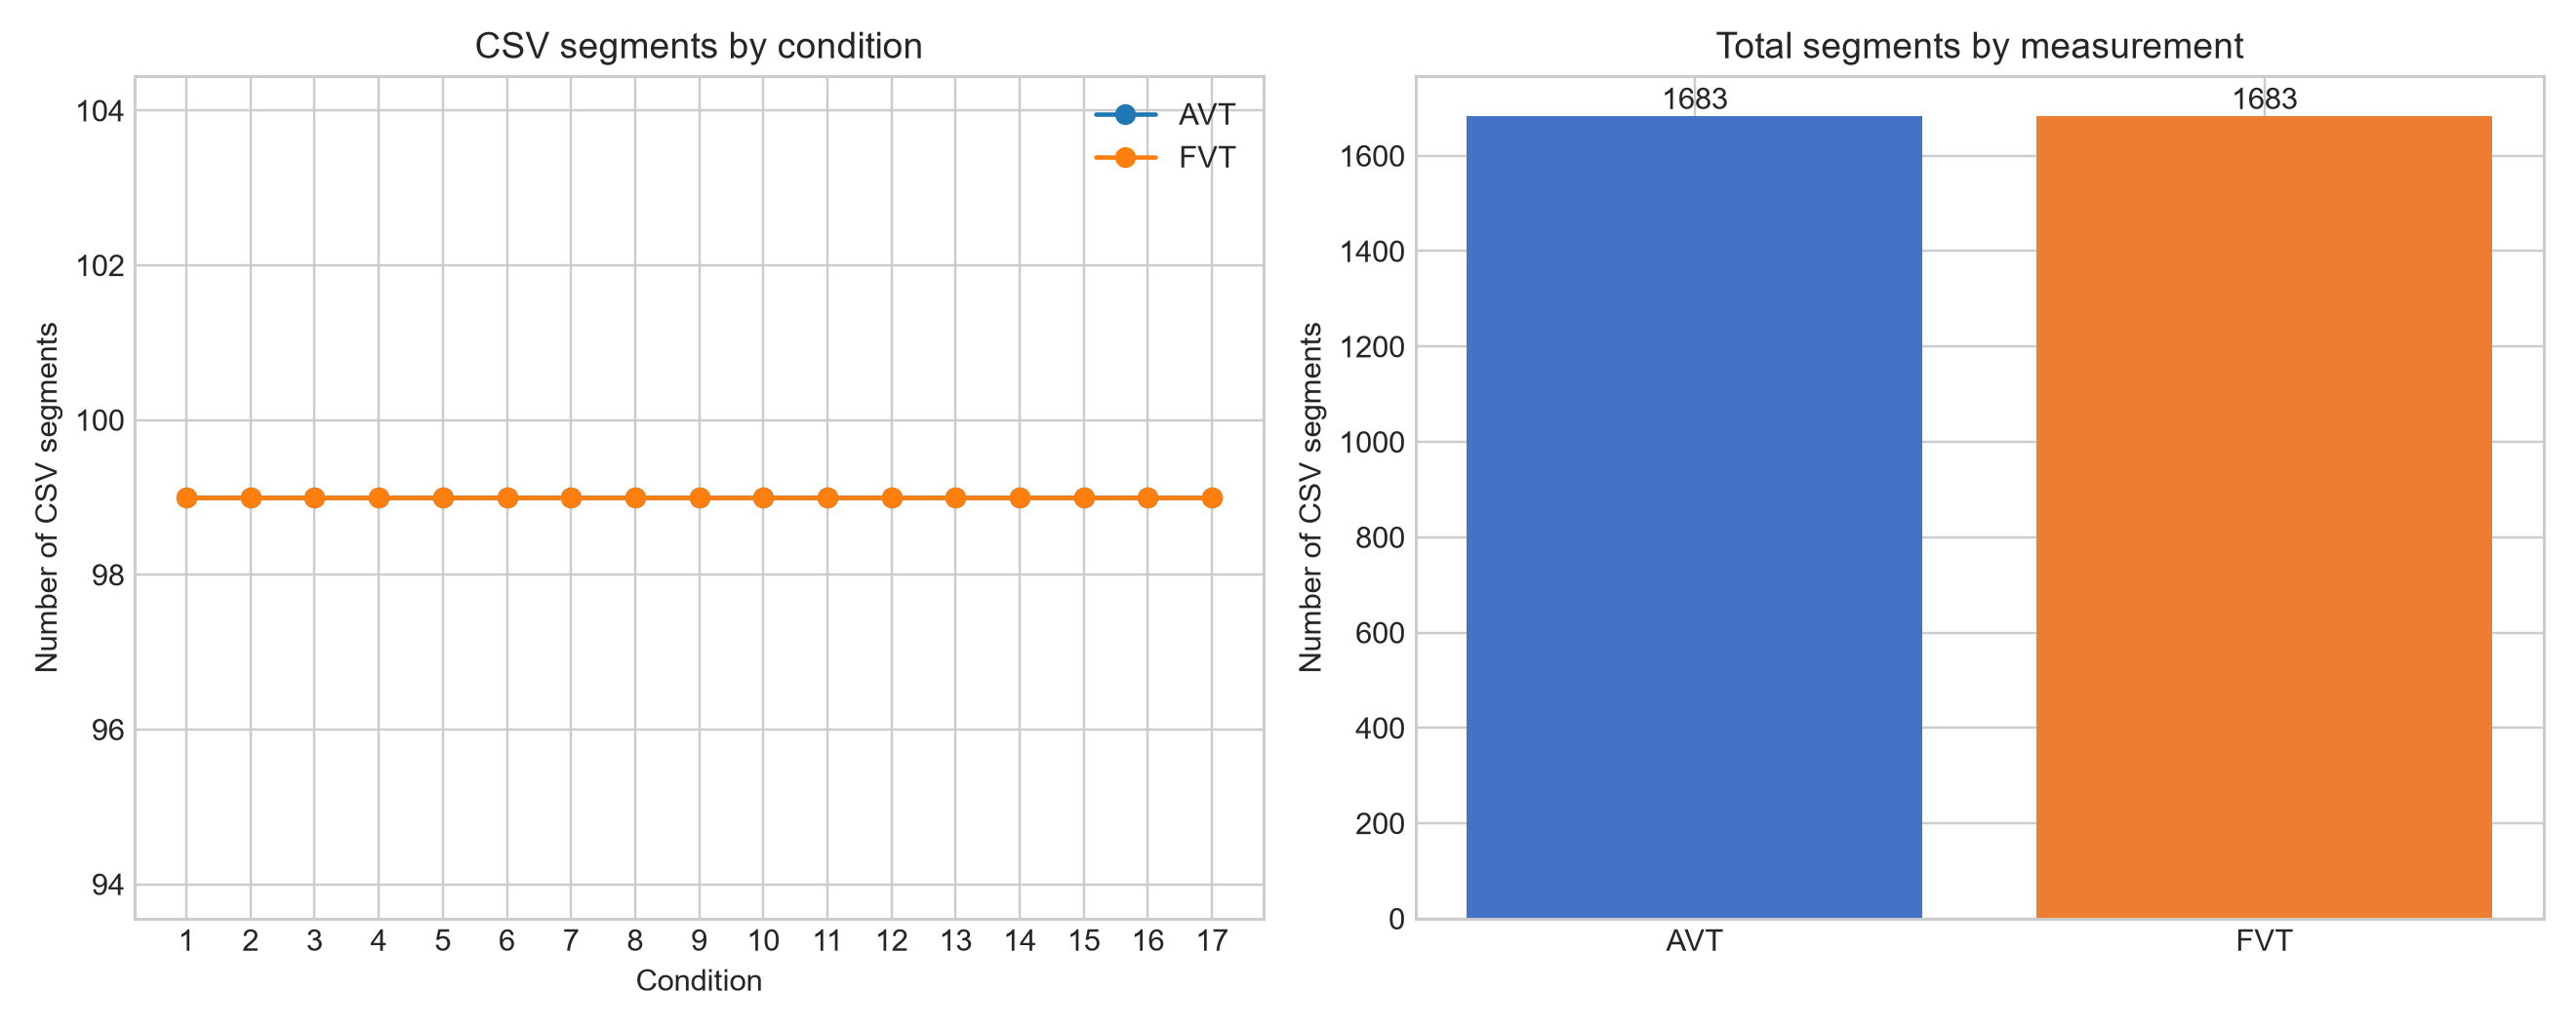
\includegraphics[width=0.96\textwidth]{img/dataset_summary.png}
\caption{CSV segment counts by condition and measurement type.}
\end{figure}

The first chart is flat at 99 segments for every condition in both AVT and FVT. The second chart shows 1,683 segments for each measurement type. This indicates balanced exported coverage: no condition has visibly fewer or more segments. These are generated segments, not fully independent observations, because ten or eleven segments from one recording remain correlated.

\begin{figure}[ht]
\centering
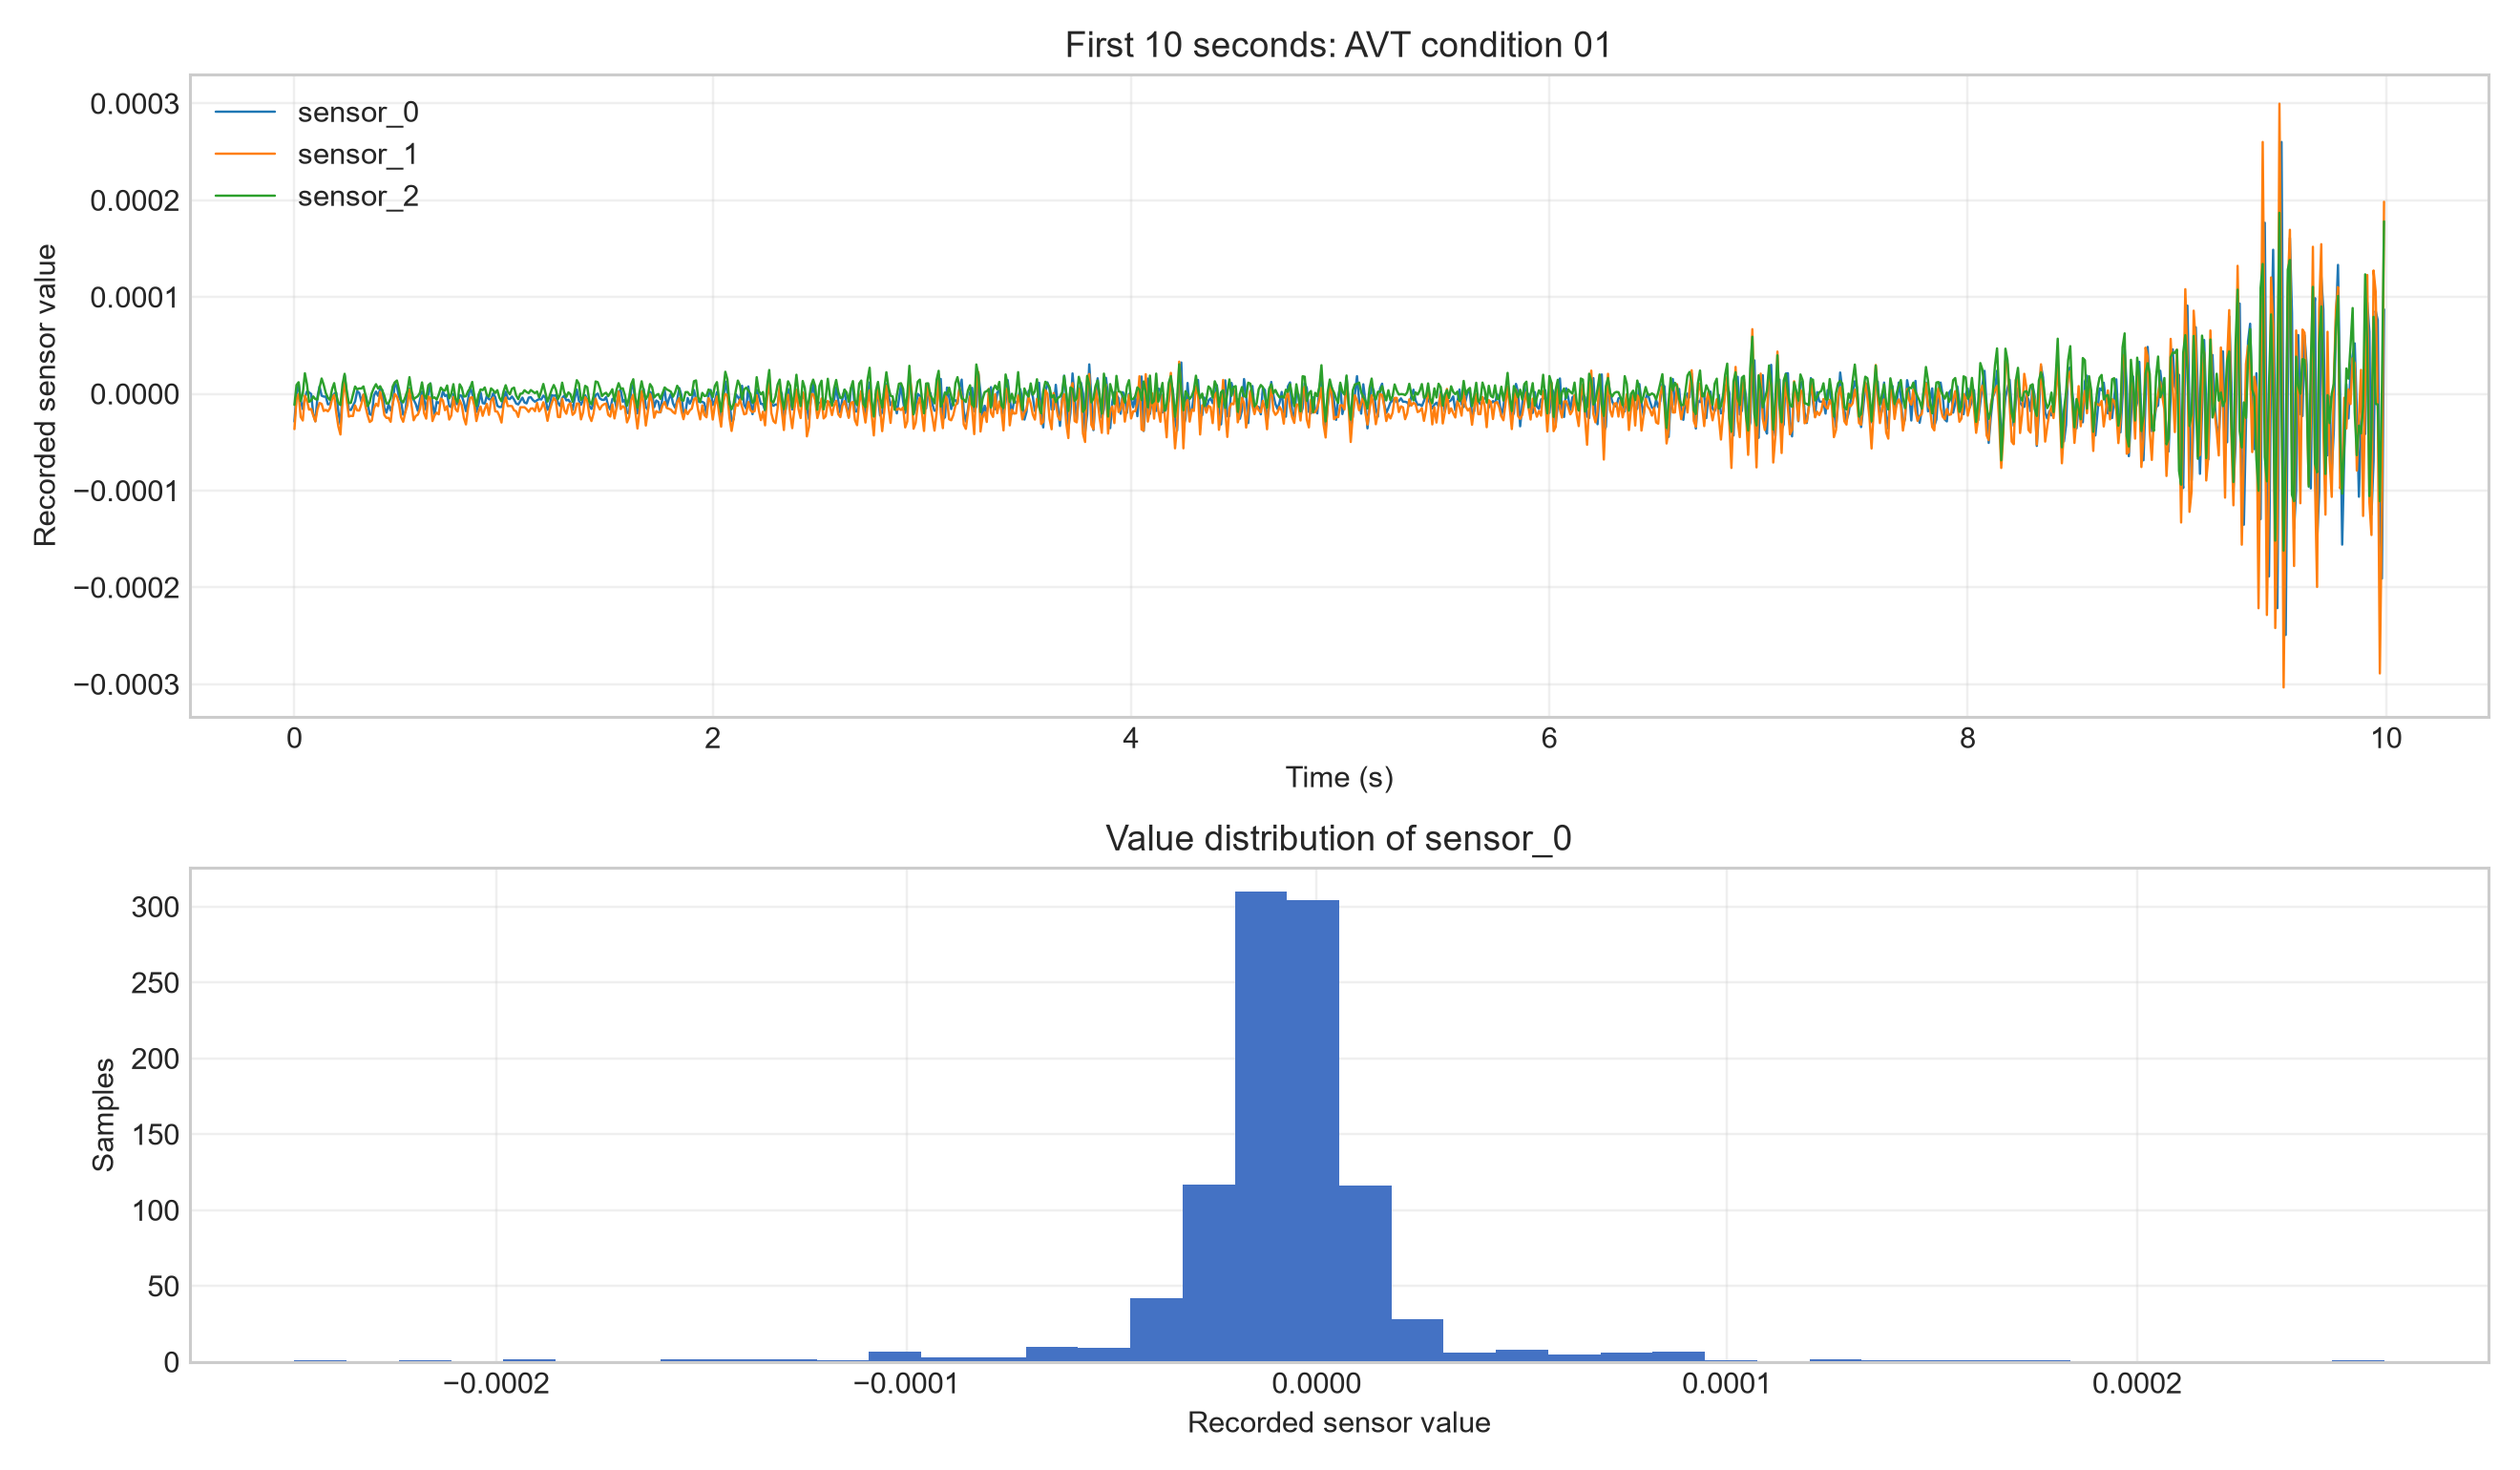
\includegraphics[width=0.96\textwidth]{img/signal_analysis.png}
\caption{Example AVT signal and sensor-0 value distribution.}
\end{figure}

The example signals oscillate near zero, which is consistent with vibration data. Their amplitude increases toward approximately 8--10 seconds and several short transients appear. A vehicle crossing or another dynamic load could explain this increase, but the chart alone cannot prove the event without a synchronized acquisition log. The histogram is concentrated near zero with small tails, meaning that most samples have low amplitude while a smaller number represent stronger transients. No missing or infinite values are visible in the plotted segment.

\section{Conclusion and next steps}
The implementation now converts the nested PDT MATLAB recordings into labeled, traceable CSV time series. The function-level flow is explicit, both AVT and FVT are stored in separate timestamped runs, and all finite samples are retained. The next steps are to verify sensor units and setup consistency, choose whether AVT and FVT will be modeled separately, split data by recording or setup to prevent leakage, normalize from the training subset only, and construct fixed-length tensors for the classifier.

\end{document}
